\section{Extracting Cross Sections}

The formula of cross section as a function of $x_{bj}$ is written as following:

\begin{equation}
 \frac{d\sigma}{d\Omega dE'}(x_{bj}^{i}) = \frac{N_{EX}^{i} \epsilon_{pion\_rej}}{N_{tg} N_{e} \epsilon_{det} \epsilon_{track}} \frac{N_{MC}^{gen}}{N_{MC}^{i} \Delta\Omega_{MC} \Delta E'_{MC}},
\label{xs_eq}
\end{equation}

where each quantities will be discussed individually in the following sections.

A package of inclusive electrons scattering cross section extraction has been developed for E08-014 experiment data. The basic structure of the code and files can be viewed from the chart bellow.

\begin{figure}[h!]
 \centerline{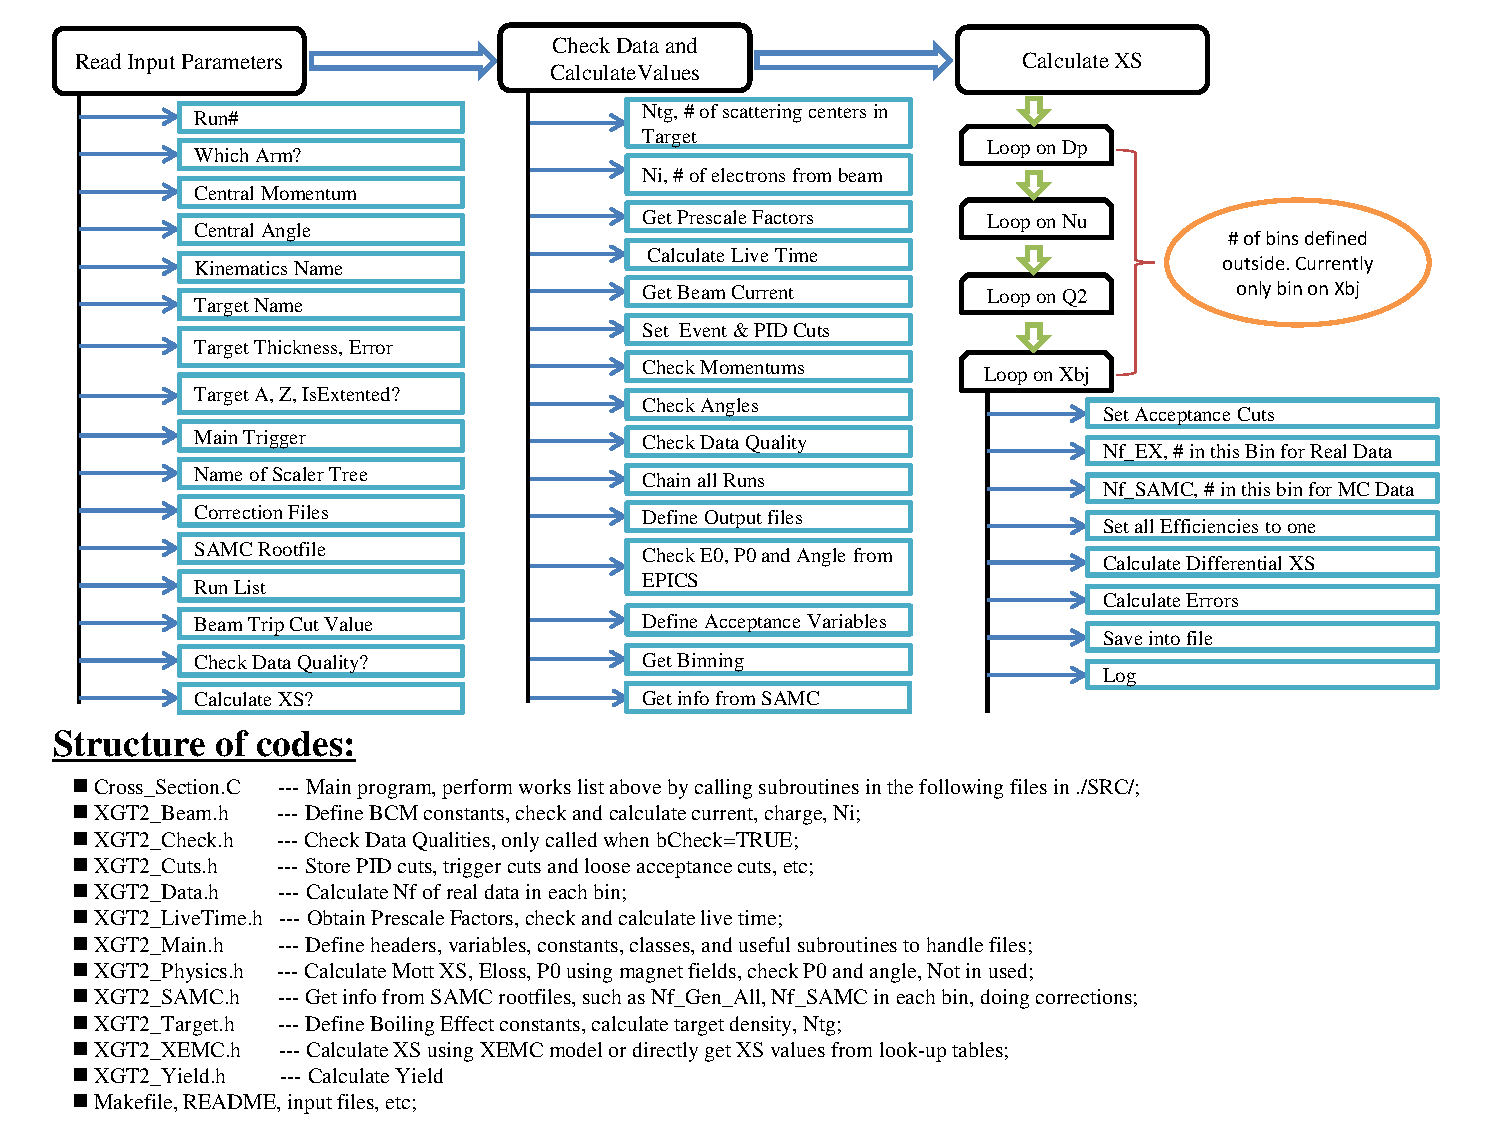
\includegraphics[width=0.95\linewidth]{./figures/XS_Chart}}
 \caption[Basic structure of XS package]{Basic structure of the cross section extraction package}
 \label{xs_chart}
\end{figure}

\subsection{Live Time}

DAQ running at high trigger rates generally decrease live time, or in other words,increases dead time. Dead time is mainly composed of hardware dead time and electronic dead time. Hardware dead time comes from the fact that detectors can not separate two or more particles coming near at the same time. Electronic dead time, which is the major source, arises when electronic modules, including computer system, skip the next event when they are still processing the current event, and cause those events not recorded by DAQ system. To reduce dead time we assign a presclae factor to each trigger type to control the total trigger rates. The values of pre-scale factors are stored in each run and can be read out to calculate the actually total number of events for different types. 

We can evaluate the electronic dead time by using the fact that events not recorded by DAQ are still counted by scalers. For each trigger type in each run, the value of live time is given by the ratio of total number of events recorded by DAQ timed the prescale factor and the total counts in scalers:

\begin{equation}
  lt_{T_{i}} = \frac{N_{T_{i}}^{DAQ} PS_{T_{i}}}{N_{T_{i}}^{Scaler}},
\end{equation}

where $N_{T_{i}}^{DAQ}$ and $N_{T_{i}}^{Scaler}$ are total number of DAQ events and scaler counts in one run after removing events taking during beam trip.

\subsection{Monte Carlo Simulation}

A simulation package, Hall-A Single Arm Monte Carlo (SAMC), which was originally developed by A. Deur \cite{} using FORTRAN and then converted into C++ by Huan Yao \cite{}, is used to study the acceptance effect of HRSs and perform cross section corrections. For each simulation event, its quantities on target plane, $x_{tg},y_{tg}, \theta_{tg}, \phi_{tg}$ and $\delta p_{tg}$, are uniformly generated in a wide phase space. A forward transportation function defines the  geometry of each HRS and transports the target variables to the focal plane if this event pass through. The calculated focal plane variables are further smeared by introducing VDCs' resolutions, then reconstructed back to the target plane  using a back-forward transportation function. Meanwhile, physics quantities, including cross sections, are also calculated for each event. The distribution of reconstructed target plane variables are compared with experiment data to verify the simulation performance. Fig~\ref{samc_tg} compare the distribution of target plane variables between simulation data and experiment data for $^{12}C$ and $^{3}He$, where for simulation data all distributions are weighted by cross sections. Note that for $^{3}He$ target, the well known bump on the vertex distribution can be seen clearly when comparing with simulation data.

\begin{figure}[!h]
 \begin{center}
 \subfloat[$^{12}C$]{
  \includegraphics[type=pdf, ext=.pdf,read=.pdf,width=0.45\textwidth]{./figures/samc/C12_Com_TG}
 } 
 \subfloat[$^{3}He$]{
  \includegraphics[type=pdf, ext=.pdf,read=.pdf,width=0.45\textwidth]{./figures/samc/He3_Com_TG}
}
 \caption[Comparing MC data and experiment data]{Comparing target plane variables of MC data (blue) and experiment data (red)}
 \label{samc_tg}
\end{center}
\end{figure}


We generate 5 million events which passing through HRSs for each target in each kinematics setting. Since calculating the radiated cross section value for each event takes extreme long time, we used XEMC cross section package to generate cross section tables for all kinematics settings and look up cross section values from the tables when we further study the simulation data. Detail discussion on XEMC will be discussed in next section. In Eq~\eqref{xs_eq}, $N_{MC}^{gen}$ is equal to total number of events generated in the entire phase space, $\Delta\Omega_{MC}\Delta E'_{MC}$, which is slightly larger than the true coverage of HRSs ($\Delta\delta p=0.12, \Delta\theta_{tg}=0.18, and \Delta\phi_{tg}=0.09$). $N_{MC}^{i}$ is the total number of events in $i$th bin that passing through acceptance cuts of each HRS and being weighted by cross section:

\begin{equation}
  N_{MC}^{i} = \sum_{j\in i} \frac{\sigma_{MC}(E_{0}^{j},E_{p}^{j},\theta^{j})}{\sigma_{MC}(E_{0}^{j},E_{p}^{j},\theta_{0})},
\end{equation}

where $\sum_{j\in i}$ means summarizing all events in $i$th bin,$\sigma_{MC}(E_{0}^{j},E_{p}^{j},\theta^{j})$ is the cross section value for $j$th event, where $E_{0}^{j}$ and $E_{p}^{j}$ are incident and outgoing energies corrected by energy loss, and $\sigma_{MC}(E_{0}^{j},E_{p}^{j},\theta_{0})$ is the cross section value at the central angle $\theta_{0}$. The ratio of $\frac{\sigma_{MC}(E_{0}^{j},E_{p}^{j},\theta^{j})}{\sigma_{MC}(E_{0}^{j},E_{p}^{j},\theta_{0})}$ will automatically do the bin-centering corrections. And $\frac{N_{MC}^{gen}}{N_{MC}^{i} \Delta\Omega_{MC} \Delta E'_{MC}}$ should be able to correct acceptance effects.


\subsection{Cross Section Model}

\subsubsection{XEMC Model} 
 To be added ...

\subsubsection{Cross Section Lookup Tables} 
 In each kinematics settings for each target, we separated a large phase space ($\Delta\delta p=0.14$ and $\Delta\theta=0.20$) into $200 \times 200$ lattices and calculated a radiated cross section value in each lattice point. The results were saved into an ascii text file. Since the bin size is fine enough, we can assume that in each $\delta p$ bin, the values of cross section does not vary too much for difference $\theta$ values, and meanwhile, in each $\theta$ bin, the distribution of cross section as function of $\delta p$ (or $E_{p}$) can be considered to be linear. Base on this assumption, for an event with ($E_{p}, \theta$), we look up the table (Fig~\ref{xs_table}), search for the most close angle value, $\theta^{i}$, as well as two momentum values,$E_{p}^{j}$ and $E_{p}^{j+1}$ (so $E_{p}^{j}<E_{p}<E_{p}^{j+1}$). We can obtain the estimated cross section value for this event using the linear relationship:

\begin{equation}
 \sigma(E_{p},\theta) = \sigma(E_{p}^{j},\theta^{i}) - \frac{E_{p}-E_{p}^{j}}{E_{p}^{j+1}-E_{p}^{j}}(\sigma(E_{p}^{j},\theta^{i})-\sigma(E_{p}^{j+1},\theta^{i}))
\end{equation}
 
We compared the difference between the table-lookup method and direct calculation, which is less than 0.1\%. 

\subsection{Acceptance and Binning}

\subsubsection{Acceptance Study}
To be added ...

\subsubsection{Binning}
In the code we prepare four variables for binning, $\delta p, \nu, Q^{2}$ and $x_{bj}$, and we can decide which one to use as well as its bin size using a input file outside the code.  We currently only bin on $x_{bj}$ with fix bin size, the value of which for each target depends on kinematics range and statistics, and which could be from 0.01 to 0.1. We used the variable calculated in the physics module in ANALYZER, such as $EKL.x\_bj$ for HRS-L, and defined a binning cut to obtain events inside the $i$th bin:

\begin{equation*}
  |EK.x\_bj - x_{bj}^{i}| <= \Delta_{bin\_size}, \qquad where x_{bi}^{i} = x_{bj}^{min} + (i+1/2)\Delta_{bin\_size}
\end{equation*}
 
\subsection{Events Selections}
  
There are several cuts applied to select good scattered electron events, for example, for events in HRS-L:

\begin{enumerate}
\item \textbf{$DBB.evtypebits>>3\&1$}, cut on trigger events, $1$ for HRS-R and $3$ for HRS-L\\
\item \textbf{$DBB.edptl[0]==0$}, remove pulse events generated by EDTM modules
\item \textbf{$L.tr.n==1$}, only allow events with one track in VDCs \\
\item \textbf{$|x_{fp}|<=0.75 \&\& |y_{fp}|<=0.55 \&\& |\theta_{fp}|<=0.15 \&\& |\phi_{fp}|<=0.045$}, focal plane acceptance cuts \\
\item \textbf{$|\delta p_{tg}|<=0.03 \&\& |ReactPointZ|<=0.07 \&\& |\theta_{tg}|<=0.03 \&\& |\phi_{tg}|<=0.02$}, target plane acceptance cuts \\
\item \textbf{$L.cer.asum\_c>=50 \&\& epL<=0.5 \&\& L.prl2.e<=100$}, PID cuts for gas Cherekov detectors, and $E/P$ and second layer of calorimeters \\
\item \textbf{$left\_current >= I_{trip}$}, beam trip cuts \\
\item Binning Cuts
\end{enumerate}

The total number of events for a list of runs after the cuts defined above is given by:

\begin{equation}
  N_{EX}^{i} = \sum_{r} \frac{N_{T_{i}}^{r} PS_{T_{i}}^{r}}{lt_{T_{i}}^{r}},
\end{equation}

where $T_{i}$ defines the type of trigger we are interested in, $r$ represents one of runs in the list, $PS_{T_{i}}^{r}$ is the pre-scale factor of this trigger, and $N_{T_{i}}^{r}$ is the total number of events from $T_{i}$ and recorded by DAQ after cutting out beam trip. 

\subsection{Evaluation of Errors}

To be added ...

\subsection{Cross Section Results}

To be added ...

\subsection{Discussion and Conclusion}

To be added ...

\end{document}

